\chapter{The MOS transistor}
\section{Symbols}
The symbols used to draw n and p MOS transistors in digital electronics are the one show in figure below

\centering
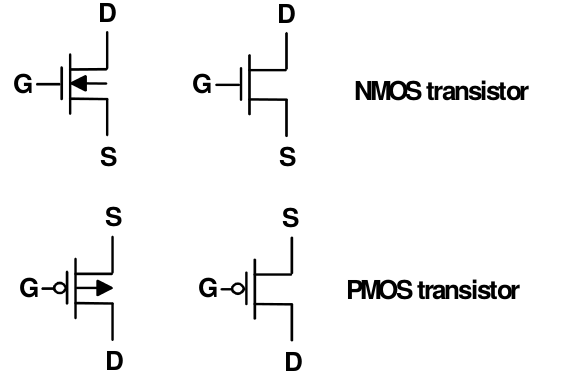
\includegraphics[width=0.35\textwidth]{C2_1.png}\\
\raggedright



\section{Working regimes}
We are intrested in the use of MOS transistors as swithces and not as amplifiers.\\
In our analysis we will consider the following operating regions with the corrisponding voltages 

\centering
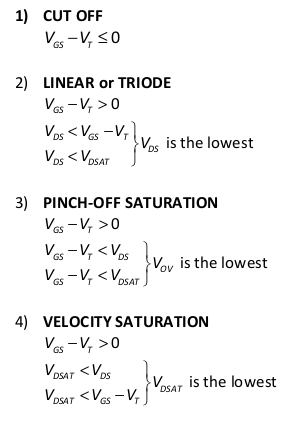
\includegraphics[width=0.3\textwidth]{C2_2.png}\\
\raggedright

and to assest the right expression of the current we will use the following unified model 


\centering
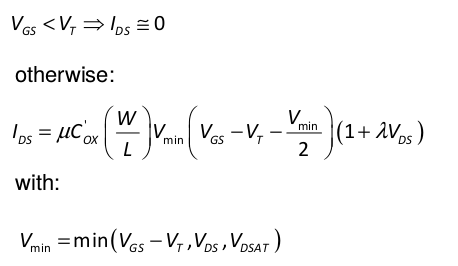
\includegraphics[width=0.5\textwidth]{C2_3.png}\\
\raggedright

In the reference technology of this course (bulk CMOS 0.25$\mu m$) this are the characteristics parameters

\centering
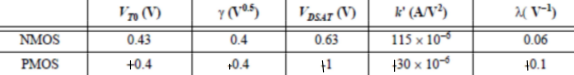
\includegraphics[width=0.7\textwidth]{C2_4.png}\\
\raggedright

\subsection{Body effect}

Since the $V_t$ depends on the source-body potential if this value is different form 0 we get

\centering
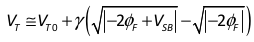
\includegraphics[width=0.35\textwidth]{C2_5.png}\\
\raggedright

where $\gamma$ is the body effect coefficient.

\subsection{Subthreshold regime}

When the overdrive voltage is equal to 0 the current in the device is not exactly 0 but the device enters in the so called subthreshold regime where the current behaves like in an BJT junction 

\centering
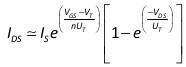
\includegraphics[width=0.35\textwidth]{C2_6.png}\\
\raggedright

this current is crucial in the power consumption in off mode.\\

\section{Equivalent resistance}
We can define an equivalent resistance of the MOS transistor as

\centering
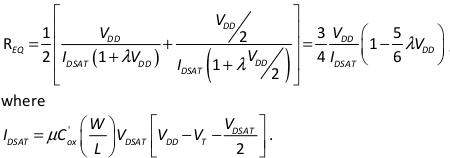
\includegraphics[width=0.5\textwidth]{C2_7.png}\\
\raggedright

the last term in parentesis can be easily neglected since is $\simeq 1$.\\
We can make three considerations:\\
\tab 1)the resistance is inversely proportional to the (W/L) ratio of the device\\
\tab 2)for $V_{DD} >> V_T + V_{DSAT}/2$, the resistance becomes virtually independent of the supply voltage\\
\tab 3)once the supply voltage approaches $V_{TE} =0.745V=V_T+V_{DSAT}/2$, a dramatic increase in resistance can be observed,even if the model adopted (considering the velocity saturation) is no longer valid\\
\vspace{5mm}
In digital electronics once we have the equivalent resistance of the MOS, we can evaluate the propagation time on the basis of the RC model, as $\ln(2)RC$.\\














